\documentclass[UTF8]{article}
%\renewcommand\abstractname{Abstract}
%\renewcommand\contentsname{Content}
%\renewcommand{\thetable}{}
\usepackage{CTEX}
\usepackage{CJKutf8}
\usepackage{fancyhdr}
\pagestyle{fancy}
\lhead{}
\chead{}
\rhead{}
\lfoot{C6600}
\cfoot{\small\sffamily 第\thepage页\quad 共\pageref{LastPage}页}
\rfoot{MathorCup2018}
\usepackage[russian]{babel}
\let\captionsrussian\empty
\let\daterussian\empty
\usepackage{caption}
\usepackage{subfigure}
\usepackage[explicit]{titlesec}
\usepackage{lastpage}
\usepackage{listings}
\usepackage{color}
\usepackage{hyperref}
\hypersetup{colorlinks=true,linkcolor=black}
\definecolor{dkgreen}{rgb}{0,0.6,0}
\definecolor{gray}{rgb}{0.5,0.5,0.5}
\definecolor{mauve}{rgb}{0.58,0,0.82}
\lstset{ %
  language=Octave,                % the language of the code
  basicstyle=\footnotesize,           % the size of the fonts that are used for the code
  numbers=left,                   % where to put the line-numbers
  numberstyle=\tiny\color{gray},  % the style that is used for the line-numbers
  stepnumber=2,                   % the step between two line-numbers. If it's 1, each line 
                                  % will be numbered
  numbersep=5pt,                  % how far the line-numbers are from the code
  backgroundcolor=\color{white},      % choose the background color. You must add \usepackage{color}
  showspaces=false,               % show spaces adding particular underscores
  showstringspaces=false,         % underline spaces within strings
  showtabs=false,                 % show tabs within strings adding particular underscores
  frame=single,                   % adds a frame around the code
  rulecolor=\color{black},        % if not set, the frame-color may be changed on line-breaks within not-black text (e.g. commens (green here))
  tabsize=2,                      % sets default tabsize to 2 spaces
  captionpos=b,                   % sets the caption-position to bottom
  breaklines=true,                % sets automatic line breaking
  breakatwhitespace=false,        % sets if automatic breaks should only happen at whitespace
  title=\lstname,                   % show the filename of files included with \lstinputlisting;
                                  % also try caption instead of title
  keywordstyle=\color{blue},          % keyword style
  commentstyle=\color{dkgreen},       % comment style
  stringstyle=\color{mauve},         % string literal style
  escapeinside={\%*}{*)},            % if you want to add LaTeX within your code
  morekeywords={*,...}               % if you want to add more keywords to the set
}
\usepackage{tabularx}  
\usepackage{graphicx}
\usepackage{enumerate}
\usepackage{geometry}
%\geometry{left=1cm,right=1cm,top=2cm,bottom=2cm}
\usepackage{amsmath}
\usepackage{amssymb} 
\usepackage{multicol}
\usepackage{indentfirst}
\setlength{\parindent}{2em}
\Large
\title{\textbf{陆基导弹打击航母的最优轨迹设计}}
\author{}
\date{}

\begin{document}
%\begin{CJK}{UTF8}{gkai}
\newpage
\thispagestyle{empty}
\maketitle
%\end{CJK}
\begin{abstract}
本文主要研究的是陆基导弹打击航母的最优轨迹设计问题,依次考虑了导弹运动过程中因燃料燃烧导致的质量变化以及不同海拔高度上风力的影响,建立了合理的动态优化模型,并得出误差分布函数,求出导弹的命中率。\\
\indent 我们不妨以东风-15短程弹道导弹为研究对象,使用其质量、最大推力等参数。我们将导弹发射阶段分为3个阶段:发射段、中段、末段。通过查阅资料确定导弹发射倾角,合理分析得出导弹在发射段做斜抛运动,计算得出导弹发射段终点即中段起点的位置。题目要求设计最难以被拦截的导弹弹道。因为导弹速率越快越不容易被计算出弹道,也越难被拦截,所以问题的实质是寻找一个能使导弹运动时间最短的运动轨迹,据此来设计中、末段。\\
\indent 针对问题一,航母静止,建立平面直角坐标系描述导弹运动轨迹。因为导弹质量随时间增加而单调减,Newton 方程将不再适用,使用И.В.Мещерский 方程作为代替分析导弹受力,得出燃料燃烧速率与火箭受到的推力值成正比。合理假设导弹在不解体的情况下所能承受的最大推力值作为约束条件,加上初速度、初始推力、起点和终点坐标、初始和最终质量等定解条件寻求能使目标泛函取最小值的最优解。\\
\indent 针对问题二,航母运动,建立空间直角坐标系,仿照问题一进行求解。\\
\indent 针对问题三,进行误差与命中率的分析。经过合理分析忽略影响因素较小的误差,只考虑风力。通过查阅文献得知钓鱼群岛所在地区常年刮东北西南季风,并得知风力值与海拔高度正相关,具体表达式却不是一个确定的关系。在И.В.Мещерский 方程中加上作为随机变量的风力,按照原先推力的最优解得到随机的弹道。考虑到末段制导对误差具有一定修正能力,据此来计算得出命中率为89.3\%\\
\textbf{关键词}:导弹打击航母;最优轨迹设计;变质量动力学;动态优化;误差分析。
\end{abstract}

\newpage
\thispagestyle{empty}
\begin{center}
\Large
\textbf{Optimal Trajectory Design of Ground Based Missile Against Aircraft Carrier}\\
\normalsize
\textbf{Summary}
\end{center}
\small
This paper mainly deals with the optimal trajectory design of the ground based missile against the aircraft carrier. The rational dynamic optimization model is established by considering the quality change caused by fuel combustion in the course of the missile movement and the influence of the wind at different altitudes, and the error distribution function is obtained, and the hit rate of the missile is obtained.\\
\indent We may take Dongfeng -15 short range ballistic missile as the object of analysis, and use its mass and maximum thrust. We divide the missile launching stage into 3 stages: the launching stage, the middle stage and the last stage. By consulting the data to determine the missile launching dip angle, the reasonable analysis of the missile in the launch section to do oblique motion, the end point of the missile launch section is the position of the starting point. The problem is to design the most difficult to intercept ballistic trajectory. Because the faster the missile speed is not easy to be calculated, the more difficult to be intercepted, so the essence of the problem is to find a trajectory that can make the missile have the shortest movement time, so the middle and the end are designed.\\
\indent Aims at the problem. First, the aircraft carrier is stationary, and the plane rectangular coordinate system is used to describe the trajectory of the missile. Because the quality of the missile increases monotonously with time, the equation of the Newton equation will not be applied. We can utilize И.В.Мещерский eqution as an alternative to the analysis of the force of the missile, and the fuel combustion rate is proportional to the thrust of the rocket. It is reasonable to assume that the maximum thrust value that the missile can bear in the case of disintegration is considered as the constraint condition, adding the initial velocity, the initial thrust, the starting point and the end point coordinates, the initial and the final quality to find the optimal solution that can make the target functional minimum.\\
\indent Aims at problem two, and establishes a space rectangular coordinate system to solve the problem.\\
\indent Analyzes error and hit rate for problem three. The errors that are ignored by reasonable analysis and neglecting factors are considered only by wind force. Through the literature, it is found that the area of the fishing archipelago shave north-east monsoon throughout the year, and that the wind value is positively related to the altitude, but the specific expression is not a definite relationship. A random trajectory is obtained based on the optimal solution of the original thrust, in which the wind force acting as a random variable is added to И.В.Мещерский equation. Considering that the terminal guidance has some ability to correct errors, based on the calculation, the hit rate is 89.3\%.\\
\textbf{Keywords}: Missile Attacking Aircraft Carrier; Optimal Trajectory Design; Variable Mass Dynamics; Dynamic Optimization; Error Analysis.
\normalsize

\newpage
\thispagestyle{empty}
\tableofcontents
\newpage
\setcounter{page}{1}
\section{引言}
军事是一国之命脉,而陆基弹道导弹在军事中有着举足轻重的地位。所以,提高陆基导弹发射前对准精度,简化对准流程,在战略战术部署中已经成为一项十分重要的工作。设计一套能适应复杂环境、快速发射、高精度的对准方案显得至关重要。\\
\indent 李卫平等学者在参考文献\ref{1}“基于最优打击序列的弹道导弹火力分配模型研究”中提出了最优打击序列,谭守林等学者在参考文献\ref{2}“弹道导弹打击航空母舰末制导有效区的确定与评估''中仿真模拟了弹道导弹打击航母的末段制导有效区的实验,对弹道导弹打击航空母舰的末段进行了分析。但在实际运用中,弹道导弹打击航空母舰过程中能够调控速度方向与大小的中段同样非常重要,而描述其完整弹道的简单的数学模型却不多见。合理假设以简化复杂的真实环境,从而建立数学模型,可以更直观的描述弹道导弹的打击过程。\\
\indent 本文成功建立了陆基导弹打击航母的动态优化模型。针对满足假设条件下不同运动状态的航空母舰,陆基导弹能够规划运动轨迹从而能成功击中航母。对真实的导弹导弹弹道设计亦有一定参考价值。
\section{问题重述}
\begin{enumerate}[1]
\item 建立初始状态下,反舰导弹打击航母的静态轨道模型。即\(t=0\)时,连接导弹初始位置与航母之间的轨道曲线模型。
\item 在航母按照已知条件(2)给出的航向和速度的航行状况下,设计导弹飞行的中段动态模型方程和算法步骤。中段通常以发射段的抛物线顶点为起始点。
\item 讨论你所设计的导弹打击航母的轨道曲线的误差分析和命中率分析。
\end{enumerate}

\section{假设与符号}
\subsection{假设}
\begin{enumerate}[1]
\item 将航母与导弹视为质点。将导弹视为刚体就要考虑导弹绕轴旋转的Coriolis 力、导弹的Euler 角等更加复杂的因素,不利于问题的求解。而导弹体积相对导弹发射点坐标与航母坐标的距离较小,忽略之后对导弹的命中率影响极小。航母同理。
\item 将航母所在的地球球面视为平面。根据参考文献\ref{3}我们将地球视为WGS-84椭球体,利用公式计算得到导弹发射点坐标与航母坐标的周向距离约为402.997km,约为地球平均周长的1\%,故在误差允许的范围内可将航母所在的地球球面视为平面。
\item 重力加速度视为定值。根据计算导弹最大海拔高度小于1个地球半径,经、纬度变化范围小于\(3^\circ\)。重力加速度随海拔高度、经度、纬度变化不明显。
\item 导弹发射点海拔高度和航母海拔高度都为0。导弹发射倾角为\(20^\circ\)。火箭发射倾角一般在\(10\sim20^\circ\)范围内。搭载卫星的火箭为了提高最高高度和精度发射倾角较小,搭载战斗部的火箭(俗称导弹)为了提高最大距离和机动性倾角较大。修改这些值不影响模型建立,只影响最终结果。
\item 导弹运动轨迹二阶连续可导。导弹燃烧燃料的速率连续。
\item 导弹仅由燃料和弹头组成,并保证所有燃料都可以完全燃烧提供推力。但真实情况是导弹通常会有假弹头、诱饵等部件,燃料也不能完全燃烧。
\end{enumerate}
\subsection{符号}
\begin{table}[htbp]
\centering
\caption{变量的定义}
\begin{tabular}{|c|l|}
\hline
\(t\)&时间\\
\hline
\(\textbf{r}\)&导弹矢径\\
\hline
\(m\)&导弹总质量\\
\hline
\(m_\textrm{min}\)&导弹弹头质量\\
\hline
\(u\)&单位时间内单位质量的燃料燃烧产生的推力\\
\hline
\(\textbf{F}\)&导弹的总推力\\
\hline
\(F_\textrm{max}\)&导弹能承受的最大推力值\\
\hline
\(\textbf{g}\)&重力加速度\\
\hline
\(l\)&航空母舰的长度\\
\hline
\(\textbf{p}\)&航母矢径\\
\hline
\(w\)&航母运动速率\\
\hline
\(\textbf{f}\)&风力\\
\hline
\(\rho\)&误差\\
\hline
\end{tabular}
\end{table}

\section{问题分析}
\begin{enumerate}[1]
\item 如果没有发生情报泄露,则导弹在发射段通常没有被敌方发现的可能。所以在发射段无需大量燃烧燃料以提高速率,只需按照初速度做斜抛运动到达指定高度为中段做准备即可。\\
导弹发射俯角\(\theta=90^\circ-20^\circ=70^\circ\),发射段经过时间47.94s。中段起点的海拔高度\(h=11.263\textrm{km}\),离发射点的水平距离\(d=8.198\textrm{km}\),离航母坐标的水平距离\(L=402.997\textrm{km}-d=394.799\textrm{km}\),中段起点速率\(v_0=v_x=0.171\textrm{km/s}\)。
\begin{figure}[htbp]
\small
\centering
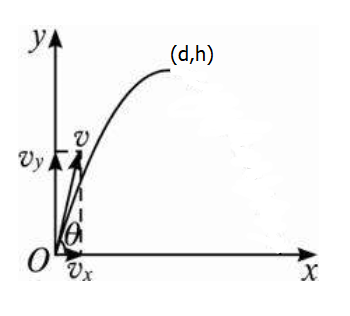
\includegraphics[width=6cm]{projectile.jpg}
\caption{斜抛运动示意图}
\end{figure}\\
题目未给出航母舰载雷达观测范围,查阅资料后知其观测半径通常为\(120\sim400\)km,而航母与导弹发射点的距离大约为400km,在最坏的情况下中段刚刚开始就已经被敌方发现。一般来说,如果导弹速度越慢,就越容易被敌方算出弹道进行拦截,所以导弹的运动轨迹应使到达航母坐标的时间越短越好,与速降线问题相似。
\begin{table}[htbp]
\centering
\caption{速降线问题与导弹命中航母问题的比较}
\begin{tabular}{|c|c|c|}
\hline
问题&速降线&导弹命中航母\\
\hline
目标泛函&时间最小&时间最小\\
\hline
起点、终点&确定&确定\\
\hline
质量&定值&随时间单调减\\
\hline
初速度&0&确定\\
\hline
受力&重力、轨道支持力&重力、燃料燃烧推力\\
\hline
\end{tabular}
\end{table}
\begin{figure}[htbp]
\small
\centering
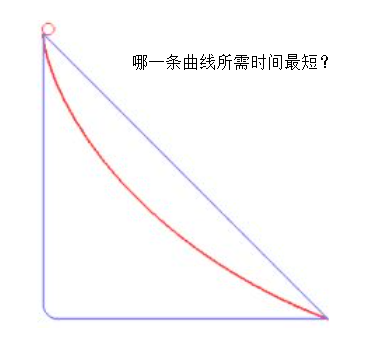
\includegraphics[width=7cm]{line.jpg}
\caption{速降线问题}
\end{figure}\\
问题一和二的区别在于航母是否运动,题目指出指挥中心可根据航母历史运动轨迹预测未来运动轨迹,问题二中航母做匀速直线运动,运动轨迹容易预测,假设预测正确,则航母的运动轨迹是完全已知的,2个模型会非常相似。
\item 前2个模型未考虑任何能引起误差的因素,如卫星和无人机定位的误差和传输信号的延迟,风力和海洋水蒸气升力。
\begin{figure}[htbp]
\small
\centering
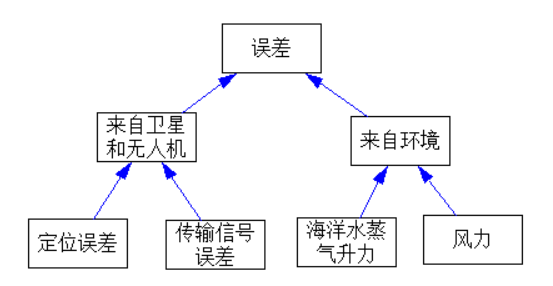
\includegraphics[width=8cm]{error.jpg}
\caption{引起误差的原因}
\end{figure}\\
查阅资料后发现现有的RTK(实时载波相位差分技术)已经能让北斗导航系统的精度达到厘米级,题目只要求米级的误差,故将其忽略不计。\\
海洋水蒸气升力在离海洋较近的范围内影响越大,离海洋距离一旦超过一个阈值几乎为0。导弹从高处发射,只有在末段才受海洋水蒸气升力影响,而末段速率较高,相对而言可忽略其影响。\\
总之,对误差影响较大的因素主要就是风力。而在末段制导时会对运动轨迹进行一定程度的修正,但修正具有一定限度。因为在前2个模型中导弹最终一定能命中航母正中心,故不妨假设修正范围即为航母长度\(l\)的一半,超过该修正范围则无法命中。据此计算出命中率。
\end{enumerate}

\section{陆基导弹打击航母的动态优化模型}
\subsection{模型的建立}
\subsubsection{航母静止}
问题一假设航母静止,在航母与导弹所在竖直平面建立平面直角坐标系,以导弹中段起点在海平面的投影为原点,以竖直向上为\(y\)轴,以海平面与航母、导弹所在竖直平面的交线为\(x\)轴,以指向航母的方向为\(x\)轴正方向。初始坐标即为\(\textbf{r}_0=(0,h)\),终点坐标即为航母坐标\(\textbf{p}_0=(L,0)\)。\\
\indent 因为导弹中段是从抛物线的最高点开始,而在该点的速度沿\(x\)轴方向,所以初速度为\(\textbf{v}_0=(v_0,0)\)。\\
\indent 初始质量为\(m_0\),为了使导弹集中航母的时间最短,应在终点燃烧导弹所有燃料,即最终导弹只剩下导弹弹头,所以终点质量必定为\(m_\textrm{min}\)。导弹一路燃烧燃料,质量随时间单调减少。\\
\indent 导弹受力没有突变,所以\(\textbf{F}(0)=\textbf{0}\)。导弹受到的推力不能大于导弹能承受的最大推力值\(F_{\textrm{max}}\),否则导弹就会有解体的可能。\\
\indent 根据动量定理的微分形式(И.В.Мещерский 方程),有
\[\textrm{d}(m\dfrac{\textrm{d}}{\textrm{d}t}\textbf{r})=\sum\textbf{F}\textrm{d}t\]
\indent 其中,\(\dfrac{\textrm{d}}{\textrm{d}t}\textbf{r}\)为速度,\(\sum\textbf{F}\)为合外力,只考虑重力和燃料燃烧产生的推力,有
\[\sum\textbf{F}=m\textbf{g}+\textbf{F}\]
\indent 两边同时除以\(\textrm{d}t\),有
\begin{equation}
m\dfrac{\textrm{d}^2}{\textrm{d}t^2}\textbf{r}+\dfrac{\textrm{d}}{\textrm{d}t}m\dfrac{\textrm{d}}{\textrm{d}t}\textbf{r}=m\textbf{g}+\textbf{F}
\label{(1)}
\end{equation}
\indent 如果考虑一个时间微元\(\textrm{d}t\),在这段时间内对导弹和燃料燃烧喷出的气体组成的整体分析动量,有
\[\Big(\big(m+\textrm{d}m\big)\big(\dfrac{\textrm{d}}{\textrm{d}t}\textbf{r}+\textrm{d}(\dfrac{\textrm{d}}{\textrm{d}t}\textbf{r})\big)-\textbf{u}\textrm{d}m\Big)-m\dfrac{\textrm{d}}{\textrm{d}t}\textbf{r}=m\textbf{g}\textrm{d}t\]
\begin{figure}[htbp]
\small
\centering
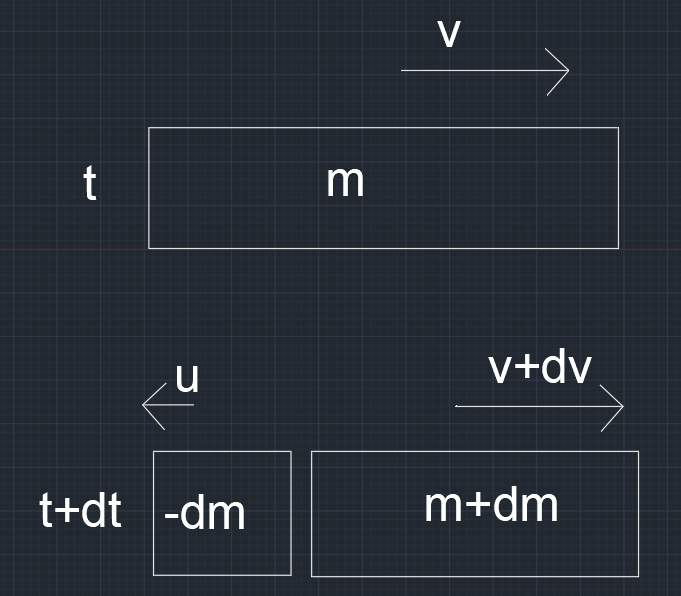
\includegraphics[width=8cm]{d.jpg}
\caption{导弹动量示意图}
\end{figure}
\indent 左式第1项是经过时间微元\(\textrm{d}t\)后的动量,第2项是之前的动量,将左式化解,两边同除以时间微元\(\textrm{d}t\),移项后有
\begin{equation}
m\dfrac{\textrm{d}^2}{\textrm{d}t^2}\textbf{r}+\dfrac{\textrm{d}}{\textrm{d}t}m\dfrac{\textrm{d}}{\textrm{d}t}\textbf{r}=m\textbf{g}+\textbf{u}\dfrac{\textrm{d}}{\textrm{d}t}m
\label{(2)}
\end{equation}
\indent 对比(\ref{(1)})和(\ref{(2)}),易得
\begin{equation}
\textbf{F}=\textbf{u}\dfrac{\textrm{d}}{\textrm{d}t}m\label{(3)}
\end{equation}
\indent 即导弹受到的推力值\(||\textbf{F}||\)与单位时间内单位质量的燃料燃烧速率\(\dfrac{\textrm{d}}{\textrm{d}t}m\)成正比,不妨设比例系数为\(u\)。根据参考文献\ref{4},\(u\)其实就是火箭燃气推进速率。对于一般的火箭发动机,\(u\)通常是常数。\\
\indent 以中段开始为时间起点,导弹的速度越快越不容易被计算出弹道,也越难被拦截,所以将目标泛函\(J\)设为经过时间\(T\)。我们的问题就是寻找一个能使时间\(T\)最小的运动轨迹\(\textbf{r}\)以及相对应的质量\(m\)和推力\(F\)。
\begin{equation}
\textrm{min }J(\textbf{r},m,\textbf{F})=T\label{(4)}
\end{equation}
\[\textrm{s. t. }\left\{
\begin{array}{l}
\textbf{r}(0)=\textbf{r}_0\\
\textbf{r}(T)=\textbf{p}_0\\
\dfrac{\textrm{d}}{\textrm{d}t}\textbf{r}(0)=\textbf{v}_0\\
m(0)=m_0\\
m(T)=m_\textrm{min}\\
\dfrac{\textrm{d}}{\textrm{d}t}m(t)\leqslant 0\\
\textbf{F}(0)=\textbf{0}\\
||\textbf{F}(t)||=-u\dfrac{\textrm{d}}{\textrm{d}t}m(t)\leqslant F_{\textrm{max}}\\
m(t)\dfrac{\textrm{d}^2}{\textrm{d}t^2}\textbf{r}(t)+\dfrac{\textrm{d}}{\textrm{d}t}m(t)\dfrac{\textrm{d}}{\textrm{d}t}\textbf{r}(t)=m(t)\textbf{g}+\textbf{F}(t)\\
\end{array}\right. \]

\subsubsection{航母运动}
问题二假设航母向南匀速直线运动。建立空间直角坐标系,以导弹中段起点在海平面的投影为原点,以竖直向上为\(z\)轴,以向南为\(x\)轴,以向东为\(y\)轴。设航母运动轨迹为\(\textbf{p}(t)=(x_0+wt,y_0,0)\)。其余条件同问题一。
\[\textrm{min }J(\textbf{r},m,\textbf{F})=T\]
\[\textrm{s. t. }\left\{
\begin{array}{l}
\textbf{r}(0)=\textbf{r}_0\\
\textbf{r}(T)=\textbf{p}(T)\\
\dfrac{\textrm{d}}{\textrm{d}t}\textbf{r}(0)=\textbf{v}_0\\
m(0)=m_0\\
m(T)=m_\textrm{min}\\
\dfrac{\textrm{d}}{\textrm{d}t}m(t)\leqslant 0\\
\textbf{F}(0)=\textbf{0}\\
||\textbf{F}(t)||=-u\dfrac{\textrm{d}}{\textrm{d}t}m(t)\leqslant F_{\textrm{max}}\\
m(t)\dfrac{\textrm{d}^2}{\textrm{d}t^2}\textbf{r}(t)+\dfrac{\textrm{d}}{\textrm{d}t}m(t)\dfrac{\textrm{d}}{\textrm{d}t}\textbf{r}(t)=m(t)\textbf{g}+\textbf{F}(t)\\
\end{array}\right. \]

\subsubsection{误差分析}
风力\(\textbf{f}\)与海拔高度、经度、纬度有关,但在一定经纬度变化较小的范围内仅与海拔高度有关,即\(\textbf{f}=\textbf{f}(\textbf{r})=\textbf{f}(z)\)。航母所在地为钓鱼群岛一带,收东北西南季风影响,不妨假定季节为夏季,风向主要为东北方向。风速随高度变化的关系是随高度增加,地面摩擦力减小,风速增加。根据参考文献\ref{5},使用幂函数作为风速随海拔高度变化的函数。因为风速具有不确定性,故将幂函数的指数设为随机变量,其分布以在参考文献\ref{6}给出的数据用幂函数拟合出的指数的均值、方差为均值、方差作正态分布。但导弹事先是无法知道风速随海拔高度变化的函数的。所以仍然让导弹沿问题2解出的控制推力\(\textbf{F}_2\)和燃料燃烧速率\(\dfrac{\textrm{d}}{\textrm{d}t}m_2\),但实际的轨迹\(\textbf{r}\)与问题2求出的理想的\(\textbf{r}_2\)有所偏差,理想的\(\textbf{r}\)与海平面交点为航母坐标,而实际的\(\textbf{r}_2\)与海平面交点与航母坐标的距离为随机变量\(\rho\),则\(\rho\)即为误差。
\[\left\{
\begin{array}{l}
m=m_2\\
\textbf{F}=\textbf{F}_2\\
m(t)\dfrac{\textrm{d}^2}{\textrm{d}t^2}\textbf{r}(t)+\dfrac{\textrm{d}}{\textrm{d}t}m(t)\dfrac{\textrm{d}}{\textrm{d}t}\textbf{r}(t)=m(t)\textbf{g}+\textbf{F}(t)+\textbf{f}(\textbf{r}(t))\\
z(T_0)=0\\
\rho=||\textbf{r}(T_0)-\textbf{p}(T_0)||\\
\end{array}\right. \]
\indent 根据问题分析,假设当\(\rho\)小于等于航母长度\(l\)的一半时即视为击中航母,则命中率为
\[\textrm{P}(A)=\textrm{P}\{\rho\leqslant\dfrac{l}{2}\}\]
\indent 事件\(A\)为导弹击中航母。

\subsection{模型的求解}
泛函(\ref{(4)})不是动态优化问题的标准形式。仿照Bernoulli 解决速降线问题的做法,对泛函(\ref{(4)})进行变形。\\
\indent 因为有约束条件
\[||\textbf{F}(t)||=-u\dfrac{\textrm{d}}{\textrm{d}t}m(t)\]
\indent 不妨设(其实就是(\ref{(3)}))
\[\textbf{F}=\textbf{u}\dfrac{\textrm{d}}{\textrm{d}t}m\]
\[||\textbf{u}||=u\]
\indent 代入И.В.Мещерский 方程,即为
\[m\dfrac{\textrm{d}^2}{\textrm{d}t^2}\textbf{r}+\dfrac{\textrm{d}}{\textrm{d}t}m\dfrac{\textrm{d}}{\textrm{d}t}\textbf{r}=m\textbf{g}+\textbf{u}\dfrac{\textrm{d}}{\textrm{d}t}m\]
\indent 令\(v=\dfrac{\textrm{d}}{\textrm{d}t}\textbf{r}\),
\[m\dfrac{\textrm{d}}{\textrm{d}t}\textbf{v}+\textbf{v}\dfrac{\textrm{d}}{\textrm{d}t}m=m\textbf{g}+\textbf{u}\dfrac{\textrm{d}}{\textrm{d}t}m\]
\[m\textrm{d}\textbf{v}+\textbf{v}\textrm{d}m=m\textbf{g}\textrm{d}t+\textbf{u}\textrm{d}m\]
\[m\textrm{d}\textbf{v}+(\textbf{v}-\textbf{u})\textrm{d}m=m\textbf{g}\textrm{d}t\]
\[\textrm{d}\textbf{v}+\frac{\textbf{v}-\textbf{u}}{m}\textrm{d}m=\textbf{g}\textrm{d}t\]
\[\textbf{v}\cdot\textrm{d}\textbf{v}+\frac{\textbf{v}\cdot(\textbf{v}-\textbf{u})}{m}\textrm{d}m=\textbf{v}\cdot\textbf{g}\textrm{d}t\]
\[v\textrm{d}v+\frac{v^2-vu\textrm{cos}\varphi}{m}\textrm{d}m=gv_y\textrm{d}t\]
\indent 其中有
\[\textbf{v}\cdot\textbf{u}=vu\textrm{cos}\varphi\]
\[\textbf{v}\cdot\textbf{g}\textrm{d}t=gv\textrm{cos}\phi=gv_y\]
\indent 至此,向量式已经被转化成了数量式。\\
\indent 同时对两边从0到\(t\)时刻积分,有
\begin{equation}
\frac{v^2}{2}-\frac{v_0^2}{2}+\int\limits_{m_0}^m\frac{v^2-vu\textrm{cos}\varphi}{\mu}\textrm{d}\mu=gy-gy_0\label{(5)}
\end{equation}
\indent 从上式中得到\(v\)满足的1个等式。
\[v=\sqrt{2\Big(gy-gy_0+\dfrac{v_0^2}{2}+\int\limits_{m_0}^m\frac{v^2-vu\textrm{cos}\varphi}{\mu}\textrm{d}\mu\Big)}\]
\indent 又因为\(v=\dfrac{\textrm{d}}{\textrm{d}t}s\),其中\(s=\sqrt{x^2+y^2}\),即\(\textrm{d}s=\sqrt{1+y'^2}\textrm{d}x\),则有
\begin{equation}
\indent v=\sqrt{1+y'^2}\dfrac{\textrm{d}}{\textrm{d}t}x\label{(6)}
\end{equation}
\indent 代入等式(\ref{(5)})即可解出\(\textrm{d}t\)。
\begin{equation}
\textrm{d}t=\sqrt{\dfrac{1+y'^2}{2\Big(gy-gy_0+\dfrac{v_0^2}{2}+\int\limits_{m_0}^m\dfrac{v^2-vu\textrm{cos}\varphi}{\mu}\textrm{d}\mu\Big)}}\textrm{d}x\label{(7)}
\end{equation}
\indent 将上式代入泛函(\ref{(4)})后化简得
\[T=\int\limits_0^T\textrm{d}t=\int\limits_{x_0}^{x_1}\sqrt{\dfrac{1+y'^2}{2\Big(gy-gy_0+\dfrac{v_0^2}{2}+\int\limits_{m_0}^m\dfrac{v^2-vu\textrm{cos}\varphi}{\mu}\textrm{d}\mu\Big)}}\textrm{d}x\]
\indent 其中,\(\textbf{r}(0)=(x_0,y_0)=(0,h)\),\(\textbf{r}(T)=(x_1,y_1)=(L,0)\),\(h\)和\(L\)的值在问题分析中已经给出。\\
\indent 至此,原来的泛函(\ref{(4)})变形为
\[\textrm{min }J(y,m,\varphi)=\int\limits_{0}^{h}\sqrt{\dfrac{1+\Big(\dfrac{\textrm{d}}{\textrm{d}x}y\Big)^2}{2\Big(gy-gh+\dfrac{v_0^2}{2}+\int\limits_{m_0}^m\dfrac{v^2-vu\textrm{cos}\varphi}{\mu}\textrm{d}\mu\Big)}}\textrm{d}x\]
\[\textrm{s. t. }\left\{
\begin{array}{l}
y(0)=h\\
y(L)=0\\
\dfrac{\textrm{d}}{\textrm{d}x}y(0)=v_0\\
m(0)=m_0\\
m(L)=m_\textrm{min}\\
\dfrac{\textrm{d}}{\textrm{d}x}m(0)=0\\
-\dfrac{F_\textrm{max}}{u}\sqrt{\dfrac{2\Big(gy-gh+\dfrac{v_0^2}{2}+\int\limits_{m_0}^m\dfrac{v^2-vu\textrm{cos}\varphi}{\mu}\textrm{d}\mu\Big)}{1+\Big(\dfrac{\textrm{d}}{\textrm{d}x}y\Big)^2}}\leqslant\dfrac{\textrm{d}}{\textrm{d}x}m\leqslant0\\
\end{array}\right. \]
\begin{figure}[htbp]
\small
\centering
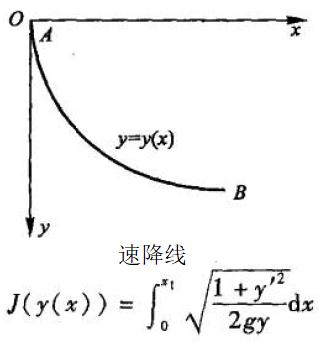
\includegraphics[width=6cm]{s.jpg}
\caption{该泛函和速降线问题的泛函有些相似}
\end{figure}
\indent 在解出\(y(x)\)、\(m(x)\)和\(\varphi(x)\)后利用等式(\ref{(3)})、(\ref{(6)})和(\ref{(7)})可求出\(m(t)\)、\(v(t)\)和\(F(t)\)。\\
\indent 因为最后1个约束条件不是普通的定解条件,所以无法直接使用古典变分法,但已经可以采用Matlab的优化工具箱求出数值解了。\\
\indent 对于问题二,在3维空间的情况更加复杂,但因为航母的匀速直线运动是已知的,可以假想有无数个导弹向航母运动轨迹的每一点发射,每条弹道都对应一个时间(导弹从发射到击中航母轨迹上的某点),航母轨迹上的每一点也都对应一个时间(航母从起点航行到该点),设以导弹中段起点在海平面的投影为端点与正东方向夹角为\(psi\)的射线与航母运动轨迹交与点\(P(\psi)\),航母运动到点\(P(\psi)\)所需时间为\(t_1(\psi)\),击中点\(P(\psi)\)的导弹经过了时间\(t_2(\psi)\),而\(t_1(\psi)\)和\(t_2(\psi)\)都是严格增的。而且在0时刻\(t_1(\psi_0)=0<t_2(\psi_0)\)。如果\(\forall\psi,t_1(\psi)<t_2(\psi)\)则导弹永远追不上航母。只需取一个较大的\(\psi\)(例如\(80^\circ\))经过计算发现先前的猜想不成立。\\
\indent 构造函数\(\tau(\psi)=t_1(\psi)-t_2(\psi)\),有\(\tau(\psi_0)<0\)和\(\tau(80^\circ)>0\),以及\(\tau\in C(\mathbb{R})\)。\\
\indent 根据连续函数的零值定理,\(\exists\psi_1,\tau(\psi_1)=0\),也就是说只要导弹沿\(\psi_1\)对应的这条射线,必能刚好在航母运动到该点时击中航母。\\
\indent 由此得出问题二中导弹的弹道其实是和问题一相同形状的平面曲线,只是导弹离航母水平距离比\(L\)大,可以用\(\psi_1\)计算得到。但为了清晰明显,我们仍然将这条平面曲线通过坐标变换画在空间直角坐标系中。容易得知\(m(t)\)、\(v(t)\)和\(F(t)\)与问题一相似,但时间更长(因为距离更远了)。
\begin{figure}[htbp]
\centering
\begin{minipage}[htbp]{7cm}
\centering
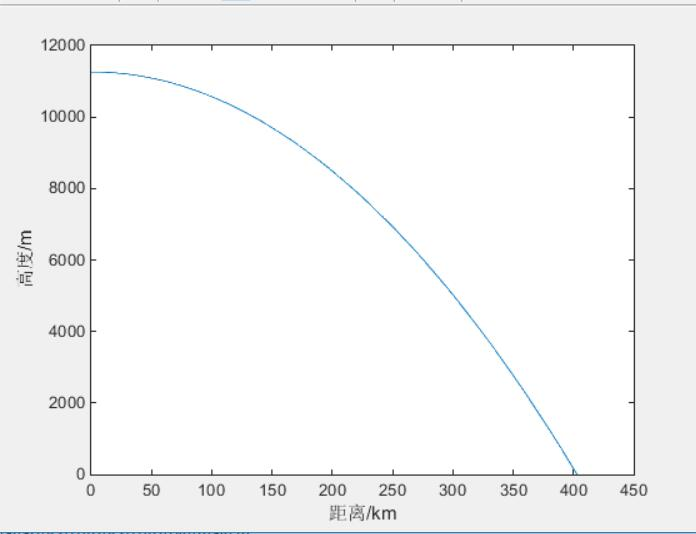
\includegraphics[width=6cm]{r1.jpg}
\caption*{子图 1:导弹中、末段运动轨迹}
\end{minipage}
\begin{minipage}[htbp]{7cm}
\centering
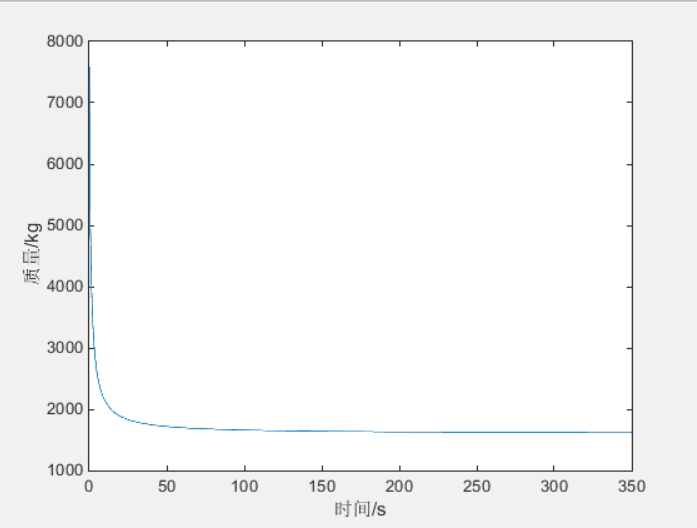
\includegraphics[width=6cm]{m1.jpg}
\caption*{子图 2:导弹中、末段质量随时间变化曲线}
\end{minipage}
\begin{minipage}[htbp]{7cm}
\centering
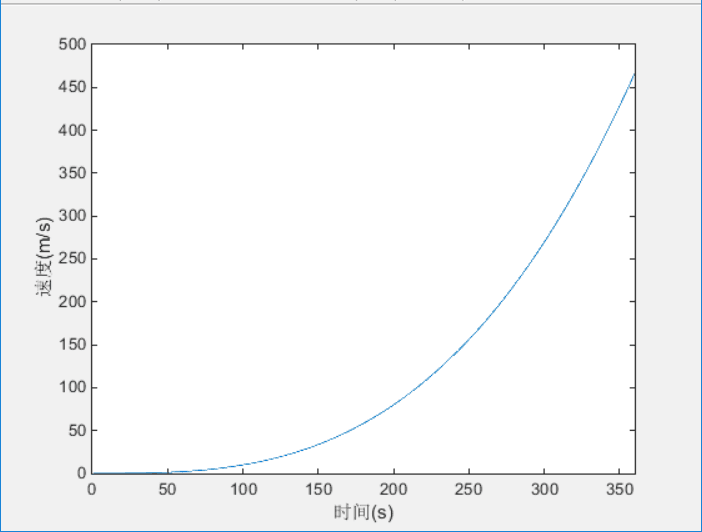
\includegraphics[width=6cm]{v1.jpg}
\caption*{子图 3:导弹中、末段速率随时间变化曲线}
\end{minipage}
\begin{minipage}[htbp]{7cm}
\centering
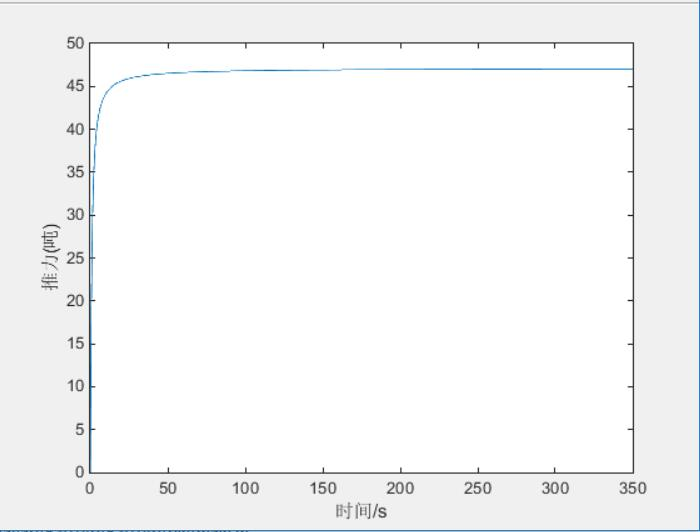
\includegraphics[width=6cm]{F1.jpg}
\caption*{子图 4:导弹中、末段推力值随时间变化曲线}
\end{minipage}
\caption{航母静止}
\end{figure}
\begin{figure}[htbp]
\centering
\begin{minipage}[htbp]{7cm}
\centering
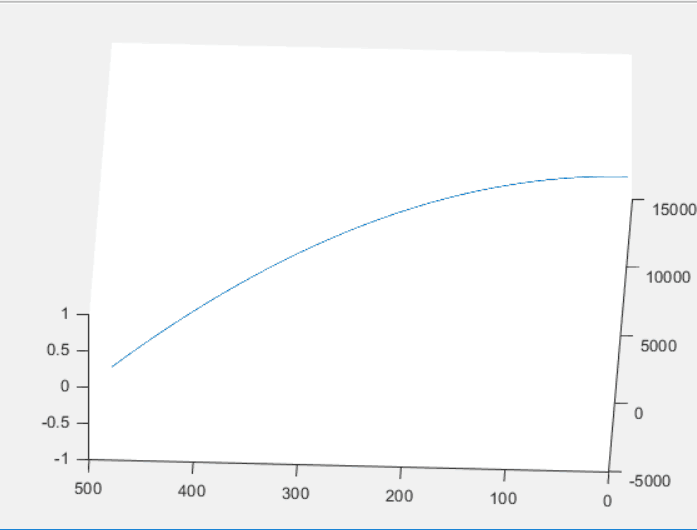
\includegraphics[width=6cm]{r2.jpg}
\caption*{子图 1:导弹中、末段运动轨迹}
\end{minipage}
\begin{minipage}[htbp]{7cm}
\centering
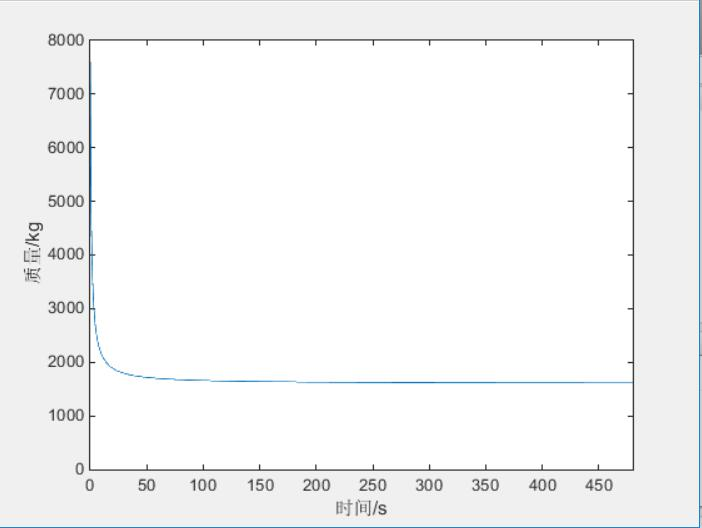
\includegraphics[width=6cm]{m2.jpg}
\caption*{子图 2:导弹中、末段质量随时间变化曲线}
\end{minipage}
\begin{minipage}[htbp]{7cm}
\centering
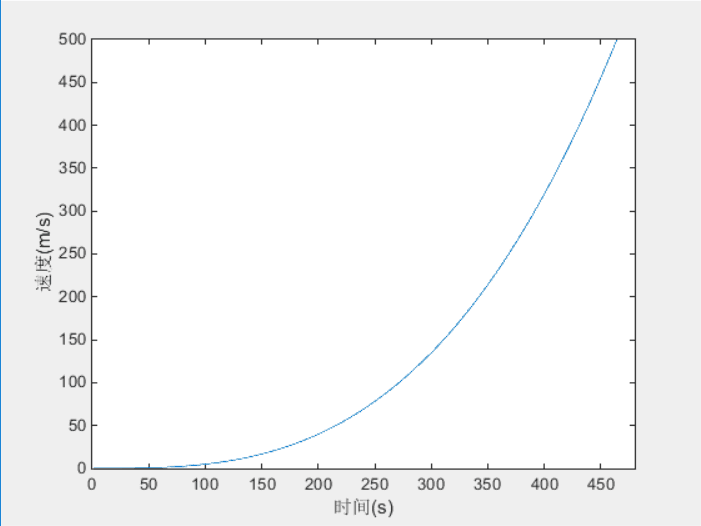
\includegraphics[width=6cm]{v2.jpg}
\caption*{子图 3:导弹中、末段速率随时间变化曲线}
\end{minipage}
\begin{minipage}[htbp]{7cm}
\centering
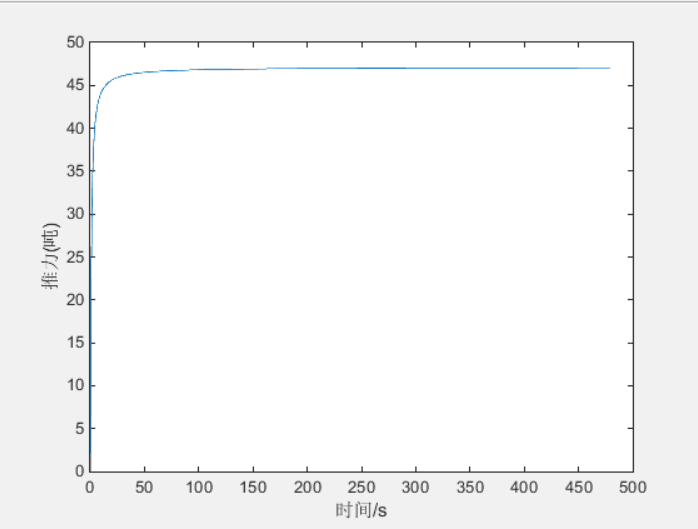
\includegraphics[width=6cm]{F2.jpg}
\caption*{子图 4:导弹中、末段推力值随时间变化曲线}
\end{minipage}
\caption{航母运动}
\end{figure}\\
\indent 容易发现在2种情况下,导弹收到的推力值都几乎在最终临近了导弹所能承受的上限。而导弹的速率则随时间单调增,在击中航母的时刻达到了最大值,并且速率曲线的斜率越来越大,因为随时间增加导弹质量单调减,推力单调增,加速率自然也会增加。导弹中段运动轨迹前期和抛物线有些相似,这是因为导弹推力值前期还不够大,对导弹运动轨迹的影响较小。推力方向比导弹指向航母的矢量方向有一个夹角,这是因为光靠重力做平抛运动所能达到的最远距离无法击中航母,所以推力的一部分与速度同向,另一部分使速度逐渐指向航母。
\begin{figure}[htbp]
\centering
\begin{minipage}[htbp]{7cm}
\centering
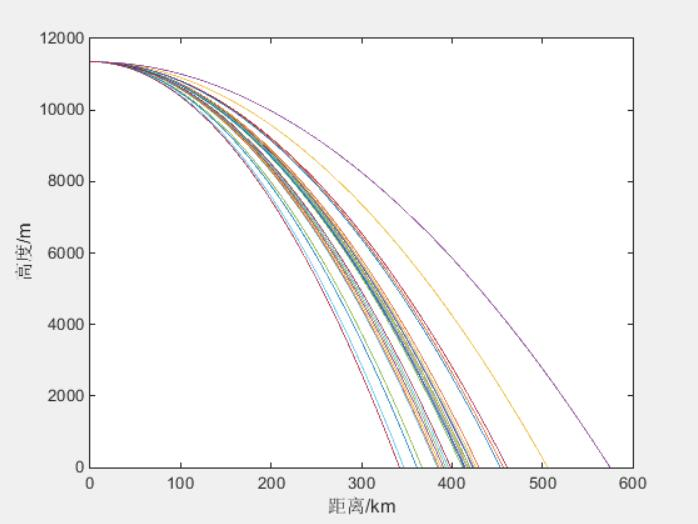
\includegraphics[width=6cm]{P.jpg}
\caption*{子图 1:导弹中段可能运动轨迹}
\end{minipage}
\begin{minipage}[htbp]{7cm}
\centering
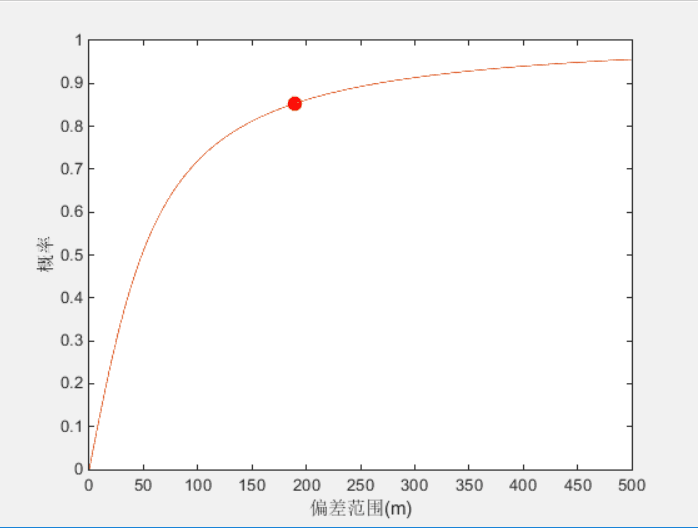
\includegraphics[width=6cm]{e.jpg}
\caption*{子图 2:误差分布函数}
\end{minipage}
\caption{误差分析}
\end{figure}\\
\indent 由于有随机变量风力的影响,导弹中、末段运动轨迹不确定。概率越大曲线族越密集。因为海拔高度较高的地方风力较大,所以曲线从一开始就出现了偏移的倾向。而从误差分布函数可以得出命中率约为89.3\%。

\subsection{灵敏度分析}
模型使用的参数众多,又因求解方法限制,无法直接画出时间\(T\)随参数变化的图像,但经过修改参数后发现灵敏度最大的参数可能是\(u\),但根据参考文献\ref{4},\(u\)变化幅度一般较小。
\indent 模型3将末段制导的误差修正能力设为航母长度的一半,但实际结果可能并非如此。在误差分布函数中可以看到误差修正能力\(x\)与命中率\(\textrm{P}(A)=\textrm{P}\{\rho\leqslant x\}\)的关系。在误差修正能力\(x\)减少较小的情况下,命中率下降并不明显。

\section{模型的评价与推广}
\subsection{优点}
\begin{enumerate}[1]
\item 本模型充分考虑了导弹在运动过程中由于燃料燃烧带来的质量变化对结果的影响,并合理忽略了导弹的形状、重力加速度的变化等因素,抓住了影响导弹运动轨迹的主要因素,既简化了模型又几乎不失其准确性。
\item 将导弹的被拦截难度用导弹的速率量化,以被舰载雷达发现后尽早击中航母为目标,使导弹运动时间最短的轨迹为最优曲线,符合实际应用。
\item 综合考虑了各种误差,选择了风力作为主要误差,并分析了命中率,得出与大多数已有论文相符的结论,可信度较高。

\end{enumerate}

\subsection{缺点}
\begin{enumerate}[1]
\item 进行了大量较强的假设,得出的曲线可能过于理想。
\item 误差和命中率分析时忽略因素过多,可能带来一定程度的误差。
\end{enumerate}

\subsection{推广}
\begin{enumerate}[1]
\item 本文提出的动态优化模型亦可被推广用于解决热气球等变质量飞行器的路径规划问题。
\item 本文提出的误差分析模型亦可以运用于跳伞运动落地点的位置预测。
\end{enumerate}

\subsection{未来的工作}
\begin{enumerate}[1]
\item 在本题的已知条件中航母的运动轨迹被指挥中心完全预测,并且航母在发现导弹后依然沿原定航道航行。未来可以考虑航母发现导弹后立即变速航行以躲避导弹追踪。这样假设之后,问题就从导弹单方的动态优化模型变成了导弹与航母双方的动态博弈模型,双方都会考虑对方的决策以做出最有利于自己的决策,从而达到均衡解。
\item 本模型进行了大量较强的假设,如果弱化这些假设可以获得比本模型更准确但也更复杂的模型。
\end{enumerate}

\newpage
\begin{thebibliography}{}
\bibitem{1}\label{1}李卫平,张海丰,孙红,李潇.基于最优打击序列的弹道导弹火力分配模型研究[J].指挥控制与仿真,2012,34(02):66-69.
\bibitem{2}\label{2}谭守林,张大巧,刁国修.弹道导弹打击航空母舰末制导有效区的确定与评估[J].指挥控制与仿真,2006(04):6-9.
\bibitem{3}\label{3}黎珍惜,黎家勋.基于经纬度快速计算两点间距离及测量误差[J].测绘与空间地理信息,2013,36(11):235-237.
\bibitem{4}\label{4}张毅,肖龙旭,王顺宏编著.弹道导弹弹道学,长沙,国防科技大学出版社,1999.3.
\bibitem{5}\label{5}王志春,宋丽莉,何秋生,刘荣,叶燕翔.风速随高度变化的曲线拟合[J].广东气象,2007(01):13-15.
\bibitem{6}\label{6}陈永利,赵永平,张必成,杨连素,吴术礼,宋珊.海上不同高度风速换算关系的研究[J].海洋科学,1989(03):27-31.
\end{thebibliography}
\addcontentsline{toc}{section}{参考文献}
\addcontentsline{toc}{section}{附录}

\begin{appendix}
\section{数据}
\begin{table}[htbp]
\centering
\caption{求解模型使用到的东风F-15的数据}
\begin{tabular}{|c|c|c|}
\hline
符号&意义&数值\\
\hline
\(m_0\)&初始质量&6200kg\\
\hline
\(m_\textrm{min}\)&弹头质量&1800kg\\
\hline
\(F_\textrm{max}\)&导弹所能承受的最大推力&450t\(\cdot g\)\\
\hline
\(u\)&火箭燃气推进速率&2\textrm{km/s}\\
\hline
\end{tabular}
\end{table}

\section{代码}
\begin{lstlisting}[title=main.m, frame=shadowbox]
clc
clear
global a b c m_0 d L p g y_2 y_og t_1 a_0 
i=1;
n=1;
    prompt = {'  a :------(o=at+a_0)--  ';'  a_0 :--';'  b:------(F=bt)--   ';'  c :------(m=m_0-ct)--   ';'  d :------(M=dm_0)--   ';'  m_0 :--';'  p :-----(p=m/l)--   ';'  L :------';'  g:--';'  pause(?) :';' hold off ( y / n ):';'   y_2 :---'};
    dlg_title = 'missile......';
    num_lines= 1;
    def     = {'-.015','.001','30','.2','6','60','1','1100','9.81','.05','y','5000'};
    inp = inputdlg(prompt,dlg_title,num_lines,def);

while(strcmp(inp,'')==0)
    hh  = strcmp(inp(11,1),'y');
    inp = str2mat( inp );
    a   = str2num(inp(1,:));
    a_0 = str2num(inp(2,:));
    b   = str2num(inp(3,:));
    c   = str2num(inp(4,:));
    d   = str2num(inp(5,:));
    m_0 = str2num(inp(6,:));
    p   = str2num(inp(7,:));
    L   = str2num(inp(8,:));
    g   = str2num(inp(9,:));
    pp  = str2num(inp(10,:));
    y_2 = str2num(inp(12,:));
    
    if(L < (m_0)/p)
       msgbox('L < l')
      break
    end
    
    % #0# 
    x_0=0 ;      y_0 = L/2-((m_0)*(L-(m_0)/p))/(2*((1+d)*m_0));    fi_0=90;   t_0=0;  m_0;

    % #1# 
    y_og1=((m_0-c*t_1)*(L-(m_0-c*t_1)/p))/(2*((1+d)*m_0-c*t_1));
    x_1=0;   y_1=L/2-y_og1;    fi_1=90;   t_1=m_0*(1+d)/(b/g+c);  m_1=m_0-c*t_1;
  
   v_22=-13/10*(1175/2+13/40*t_1)/(600-13/5*t_1)+13/40*(50-13/10*t_1)/(600-13/5*t_1)+13/5*(50-13/10*t_1)*(1175/2+13/40*t_1)/(600-13/5*t_1)^2;
   
    
    % #2#
    tt=1;
    t_2 = t_1 + tt;
    [T_2,Y_2] = ode45(@state2,[t_1 t_2],[L/2-y_og1 v_22]);
    while(Y_2(length(Y_2(:,1)),1) < (y_2 + y_1))
        tt = tt + 1;t_2 = t_1 + tt;
        [T_2,Y_2] = ode45(@state2,[t_1 t_2],[L/2-y_og1 v_22]);
        
    end
    
    x_2 = 0;       fi_2 = 90;   m_2 = m_0-c*t_2;  y_2 = Y_2(length(Y_2(:,1)),1);
    
    v_y2 = Y_2(length(Y_2(:,2)),2);
  
    if(m_2 < 0)
         msgbox('fule is low (1)')
    break
    end

    % #3#
    t_3 = m_2/c;mm=0;
tt_3=1;
    [T_3,Y_3]=ode45(@state3,[t_2 t_2+tt_3],[0 y_2 90 0 v_y2 0]);
    while((Y_3(length(Y_3(:,5)),1) > 0))
        tt_3 = tt_3 + 1;t_2 = t_1 + tt_3;
        [T_3,Y_3]=ode45(@state3,[t_2 t_2+tt_3],[0 y_2 90 0 v_y2 0]);
        mm=mm+1;
   end
    
    if(t_3 < tt_3)
         msgbox('fule is low (2)')
    break
    end
       
    x_3 = Y_3(length(Y_3(:,1)),1);
    y_3 = Y_3(length(Y_3(:,2)),2);
    fi_3 = Y_3(length(Y_3(:,3)),3);
    v_x3 = Y_3(length(Y_3(:,4)),4);
    v_y3 = Y_3(length(Y_3(:,5)),5);
    w_fi3 = Y_3(length(Y_3(:,6)),6);

    % #4#
    t_4 = m_0/c;
    [T_4,Y_4]=ode45(@state4,[t_2+tt_3 t_4],[x_3 y_3 fi_3 v_x3 v_y3 w_fi3]);
    x_4 = Y_4(length(Y_4(:,1)),1);
    y_4 = Y_4(length(Y_4(:,2)),2);
    fi_4 = Y_4(length(Y_4(:,3)),3);
    v_x4 = Y_4(length(Y_4(:,4)),4);
    v_y4 = Y_4(length(Y_4(:,5)),5);
    w_fi4 = Y_4(length(Y_4(:,6)),6);

    
    
    % #5#

    tt=1;
    [T_5,Y_5]=ode45(@state5,[t_4 t_4+tt],[x_4 y_4 fi_4 v_x4 v_y4 w_fi4]);
    while(Y_5(length(Y_5(:,2)),2) > 0)
        [T_5,Y_5]=ode45(@state5,[t_4 t_4+tt],[x_4 y_4 fi_4 v_x4 v_y4 w_fi4]);
        tt = tt +1;
        
    end
 

   plot(zeros(length(Y_2),1),Y_2(:,1)  ,Y_3(:,1),Y_3(:,2) ,'-' ,Y_4(:,1),Y_4(:,2),'--' ,Y_5(:,1),Y_5(:,2),'b--' ),xlabel('x'),ylabel('y'),grid
   pause
   
   T_1=[1:t_1];
   y_og2=L/2-((m_0-c*T_1).*(L-(m_0-c*T_1)/p))./(2*((1+d)*m_0-c*T_1)) ;
   v_2=-13./10*(1175./2+13./40.*T_1)./(600-13./5.*T_1)+13./40.*(50-13./10.*T_1)./(600-13./5.*T_1)+13./5.*(50-13./10.*T_1).*(1175./2+13./40.*T_1)./(600-13./5.*T_1).^2;
   GG=zeros(length(T_1),1);
   
   subplot(2,3,1),plot(T_1,GG,T_2,zeros(length(Y_2),1),T_3,Y_3(:,1),'-g',T_4,Y_4(:,1),'--'),ylabel('x'),xlabel('t'),grid
   subplot(2,3,2),plot(T_1,  y_og2 ,T_2,Y_2(:,1),T_3,Y_3(:,2) ,'-g',T_4,Y_4(:,2),'--'),ylabel('v'),xlabel('t'),grid
   subplot(2,3,3),plot(T_1,GG,T_2,90*ones(length(Y_2),1),T_3,Y_3(:,3),'-g',T_4,Y_4(:,3),'--'),ylabel('fi'),xlabel('t'),grid   
   subplot(2,3,4),plot(T_1,GG,T_2,zeros(length(Y_2),1),T_3,Y_3(:,4),'-g',T_4,Y_4(:,4),'--'),ylabel('dx'),xlabel('t'),grid
   subplot(2,3,5),plot(T_1,v_2,T_2,Y_2(:,2),T_3,Y_3(:,5),'-g',T_4,Y_4(:,5),'--'),ylabel('dy'),xlabel('t'),grid
   subplot(2,3,6),plot(T_1,GG,T_2,zeros(length(Y_2),1),T_3,Y_3(:,6),'-g',T_4,Y_4(:,6),'--'),ylabel('dfi'),xlabel('t'),grid


   pause
   cc=Y_3(1,2);
   i=1;
   while(abs((Y_3(i,2)-cc)) < 2)
       i=i+1;
       
   end
 
   X=[GG;zeros(length(Y_2(:,1)),1);Y_3(i:length(Y_3(:,2)),1);Y_4(:,1);Y_5(:,1)];
   Y=[y_og2;Y_2(:,1);Y_3(i:length(Y_3(:,2)),2);Y_4(:,2);Y_5(:,2)];
   FI=[90*ones(length(Y_2(:,1))+length(T_1),1) ; Y_3(i:length(Y_3(:,2)),3) ; Y_4(:,3);Y_5(:,3)];
   V_x=[GG;zeros(length(Y_2(:,1)),1);Y_3(i:length(Y_3(:,2)),4);Y_4(:,4);Y_5(:,4)];
   V_y=[v_2;Y_2(:,2);Y_3(i:length(Y_3(:,2)),5);Y_4(:,5);Y_5(:,5)];
   T=[T_1;T_2;T_3(i:length(T_3),1);T_4;T_5];
   X_max=X(1,1);   Y_max=Y(1,1); X_min=X(1,1);   Y_min=Y(1,1);
   
   for i=1:1:length(X)
       if(X(i,1) > X_max)
           X_max=X(i,1);
       end
       if(X(i,1) < X_min)
           X_min=X(i,1);
       end
       if(Y(i,1) > Y_max)
           Y_max=Y(i,1);
       end
       if(Y(i,1) < Y_min)
           Y_min=Y(i,1);
       end
   end
%-------------------------1---------------------------   
subplot(1,1,1)
for i=1:1:length(Y)
      if(T(i,1) <= (t_2 + t_3)) 
          y_og = ((m_0-c*T(i,1))*(L-(m_0-c*T(i,1))/p))/(2*((1+d)*m_0-c*T(i,1))) ;     
          L_m = (m_0-c*T(i,1))/p;
          aa = 7/200;
          L_w = (1-c*T(i,1)/(m_0*(1+d)))*L/5;
          L_F = L*b*T(i,1)/(5*m_0*(1+d)*g);
      else
          y_og=0;
          L_m=0;aa=0;
          L_w=L/(5*(1+1/d));
          L_F=0;               
      end
      if((T(i,1) <= (t_2))|(T(i,1) >= (t_2+t_3))) 
          cc=0;
      else 
          cc=a*(T(i,1)-t_2);
      end
     plot([X(i,1)-(L/2-y_og)*cos( FI(i,1)*pi/180 ),X(i,1)+(L/2+y_og)*cos( FI(i,1)*pi/180 )],[Y(i,1)-(L/2-y_og)*sin(FI(i,1)*pi/180),Y(i,1)+(L/2+y_og)*sin(FI(i,1)*pi/180)]);
     xlim([X_min - L , X_max + L])
     ylim([Y_min - L , Y_max + L])
     hold on
     XX_0 = X(i,1) - (L/2-y_og)*cos(FI(i,1)*pi/180);
     YY_0 = Y(i,1) - (L/2-y_og)*sin(FI(i,1)*pi/180);
     XX_1 = XX_0 - aa*L*sin( FI(i,1)*pi/180 );
     XX_2 = XX_1 + L_m*cos( FI(i,1)*pi/180 );
     XX_3 = XX_2 + aa*2*L*sin( FI(i,1)*pi/180 );
     XX_4 = XX_3 - L_m*cos( FI(i,1)*pi/180 );
     YY_1 = YY_0 + aa*L*cos( FI(i,1)*pi/180 );
     YY_2 = YY_1 + L_m*sin( FI(i,1)*pi/180 );
     YY_3 = YY_2 - aa*2*L*cos( FI(i,1)*pi/180 );
     YY_4 = YY_3 - L_m*sin( FI(i,1)*pi/180 );
     plot(X(i,1),Y(i,1),'+g')
     plot([XX_1,XX_2,XX_3,XX_4,XX_1],[YY_1,YY_2,YY_3,YY_4,YY_1],'r');
%fill([XX_1,XX_2,XX_3,XX_4,XX_1],[YY_1,YY_2,YY_3,YY_4,YY_1],'r');
     bb=2/15;     
%----------w
     plot([X(i,1),X(i,1)    , X(i,1)-bb*L_w/((2)^.5)     , X(i,1)-bb*L_w/((2)^.5)+(2)^.5*bb*L_w , X(i,1)],...
          [Y(i,1),Y(i,1)-L_w, Y(i,1)-L_w+bb*L_w/((2)^.5) , Y(i,1)-L_w+bb*L_w/((2)^.5)           , Y(i,1)-L_w],'k')
%----------F
    plot([XX_0 , XX_0-bb*L_F*cos((cc+FI(i,1)-45)*pi/180) , XX_0+bb*L_F*sin((cc+FI(i,1)-45)*pi/180) , XX_0 , XX_0-L_F*cos((cc+FI(i,1))*pi/180)],...
         [YY_0 , YY_0-bb*L_F*sin((cc+FI(i,1)-45)*pi/180) , YY_0-bb*L_F*cos((cc+FI(i,1)-45)*pi/180) , YY_0 , YY_0-L_F*sin((cc+FI(i,1))*pi/180)],'k')
%----------f_x
     L_vx = L/5*(sign(V_x(i,1)).*0.1.*V_x(i,1).^2)/(m_0*g*(1+d));
    plot([X(i,1) + y_og*cos( FI(i,1)*pi/180 ) , X(i,1) + y_og*cos( FI(i,1)*pi/180 ) + L_vx*bb*((2)^(.5))/2 , X(i,1) + y_og*cos( FI(i,1)*pi/180 ) + L_vx*bb*((2)^(.5))/2                      , X(i,1) + y_og*cos( FI(i,1)*pi/180 ) , X(i,1) + y_og*cos( FI(i,1)*pi/180 ) + L_vx],...
         [Y(i,1) + y_og*sin( FI(i,1)*pi/180 ) , Y(i,1) + y_og*sin( FI(i,1)*pi/180 ) + L_vx*bb*((2)^(.5))/2 , Y(i,1) + y_og*sin( FI(i,1)*pi/180 ) + L_vx*bb*((2)^(.5))/2 - bb*((2)^(.5))*L_vx , Y(i,1) + y_og*sin( FI(i,1)*pi/180 ) , Y(i,1) + y_og*sin( FI(i,1)*pi/180 )       ],'r')
%----------f_y
     L_vy = L/5*(sign(V_y(i,1)).*0.1.*V_y(i,1).^2)/(m_0*g*(1+d));
     plot([X(i,1) + y_og*cos( FI(i,1)*pi/180 ) , X(i,1) + y_og*cos( FI(i,1)*pi/180 ) - L_vy*bb*((2)^(.5))/2 , X(i,1) + y_og*cos( FI(i,1)*pi/180 ) - L_vy*bb*((2)^(.5))/2 + bb*((2)^(.5))*L_vy , X(i,1) + y_og*cos( FI(i,1)*pi/180 ) , X(i,1) + y_og*cos( FI(i,1)*pi/180 )       ]...
         ,[Y(i,1) + y_og*sin( FI(i,1)*pi/180 ) , Y(i,1) + y_og*sin( FI(i,1)*pi/180 ) + L_vy*bb*((2)^(.5))/2 , Y(i,1) + y_og*sin( FI(i,1)*pi/180 ) + L_vy*bb*((2)^(.5))/2                      , Y(i,1) + y_og*sin( FI(i,1)*pi/180 ) , Y(i,1) + y_og*sin( FI(i,1)*pi/180 ) + L_vy],'r')
     if(hh==1)
         hold off
     end
 pause(pp+.03)
end
% --------------2-----------------------------   

 for i=1:1:length(Y)
      if(T(i,1) <= (t_2 + t_3)) 
          y_og=((m_0-c*T(i,1))*(L-(m_0-c*T(i,1))/p))/(2*((1+d)*m_0-c*T(i,1))) ;     
          L_m=(m_0-c*T(i,1))/p; aa=7/200;
          L_w=(1-c*T(i,1)/(m_0*(1+d)))*L/5;
          L_F=L*b*T(i,1)/(5*m_0*(1+d)*g);
      else
          y_og=0;
          L_m=0;aa=0;
          L_w=L/(5*(1+1/d));
          L_F=0;               
      end
      if((T(i,1) <= (t_2))|(T(i,1) >= (t_2+t_3))) 
          cc=0;
      else 
          cc=a*(T(i,1)-t_2);
      end
     
    plot([X(i,1)-(L/2-y_og)*cos( FI(i,1)*pi/180 ),X(i,1)+(L/2+y_og)*cos( FI(i,1)*pi/180 )],[Y(i,1)-(L/2-y_og)*sin(FI(i,1)*pi/180),Y(i,1)+(L/2+y_og)*sin(FI(i,1)*pi/180)]);
    hold on
    xlim([X(i,1)-L X(i,1)+L])
    ylim([Y(i,1)-L Y(i,1)+L])
    XX_0=X(i,1)-(L/2-y_og)*cos(FI(i,1)*pi/180);
    YY_0=Y(i,1)-(L/2-y_og)*sin(FI(i,1)*pi/180);
    XX_1 = XX_0 - aa*L*sin( FI(i,1)*pi/180 );
    XX_2 = XX_1 + L_m*cos( FI(i,1)*pi/180 );
    XX_3 = XX_2 + aa*2*L*sin( FI(i,1)*pi/180 );
    XX_4 = XX_3 - L_m*cos( FI(i,1)*pi/180 );
    YY_1 = YY_0 + aa*L*cos( FI(i,1)*pi/180 );
    YY_2 = YY_1 + L_m*sin( FI(i,1)*pi/180 );
    YY_3 = YY_2 - aa*2*L*cos( FI(i,1)*pi/180 );
    YY_4 = YY_3 - L_m*sin( FI(i,1)*pi/180 );
    plot(X(i,1),Y(i,1),'+g')
    plot([XX_1,XX_2,XX_3,XX_4,XX_1],[YY_1,YY_2,YY_3,YY_4,YY_1],'r');
%fill([XX_1,XX_2,XX_3,XX_4,XX_1],[YY_1,YY_2,YY_3,YY_4,YY_1] ,'r');
  bb=2/15;
%----------w
     plot([X(i,1),X(i,1)    , X(i,1)-bb*L_w/((2)^.5)     , X(i,1)-bb*L_w/((2)^.5)+(2)^.5*bb*L_w , X(i,1)],...
          [Y(i,1),Y(i,1)-L_w, Y(i,1)-L_w+bb*L_w/((2)^.5) , Y(i,1)-L_w+bb*L_w/((2)^.5)           , Y(i,1)-L_w],'k')
%----------F
     plot([XX_0 , XX_0-bb*L_F*cos((cc+FI(i,1)-45)*pi/180) , XX_0+bb*L_F*sin((cc+FI(i,1)-45)*pi/180) , XX_0 , XX_0-L_F*cos((cc+FI(i,1))*pi/180)],...
          [YY_0 , YY_0-bb*L_F*sin((cc+FI(i,1)-45)*pi/180) , YY_0-bb*L_F*cos((cc+FI(i,1)-45)*pi/180) , YY_0 , YY_0-L_F*sin((cc+FI(i,1))*pi/180)],'k')
%----------f_x
     L_vx = L/5*(sign(V_x(i,1)).*0.1.*V_x(i,1).^2)/(m_0*g*(1+d));
     plot([X(i,1) + y_og*cos( FI(i,1)*pi/180 ) , X(i,1) + y_og*cos( FI(i,1)*pi/180 ) + L_vx*bb*((2)^(.5))/2 , X(i,1) + y_og*cos( FI(i,1)*pi/180 ) + L_vx*bb*((2)^(.5))/2                      , X(i,1) + y_og*cos( FI(i,1)*pi/180 ) , X(i,1) + y_og*cos( FI(i,1)*pi/180 ) + L_vx],...
          [Y(i,1) + y_og*sin( FI(i,1)*pi/180 ) , Y(i,1) + y_og*sin( FI(i,1)*pi/180 ) + L_vx*bb*((2)^(.5))/2 , Y(i,1) + y_og*sin( FI(i,1)*pi/180 ) + L_vx*bb*((2)^(.5))/2 - bb*((2)^(.5))*L_vx , Y(i,1) + y_og*sin( FI(i,1)*pi/180 ) , Y(i,1) + y_og*sin( FI(i,1)*pi/180 )       ],'r')
%----------f_y
     L_vy = L/5*(sign(V_y(i,1)).*0.1.*V_y(i,1).^2)/(m_0*g*(1+d));
     plot([X(i,1) + y_og*cos( FI(i,1)*pi/180 ) , X(i,1) + y_og*cos( FI(i,1)*pi/180 ) - L_vy*bb*((2)^(.5))/2 , X(i,1) + y_og*cos( FI(i,1)*pi/180 ) - L_vy*bb*((2)^(.5))/2 + bb*((2)^(.5))*L_vy , X(i,1) + y_og*cos( FI(i,1)*pi/180 ) , X(i,1) + y_og*cos( FI(i,1)*pi/180 )       ]...
         ,[Y(i,1) + y_og*sin( FI(i,1)*pi/180 ) , Y(i,1) + y_og*sin( FI(i,1)*pi/180 ) + L_vy*bb*((2)^(.5))/2 , Y(i,1) + y_og*sin( FI(i,1)*pi/180 ) + L_vy*bb*((2)^(.5))/2                      , Y(i,1) + y_og*sin( FI(i,1)*pi/180 ) , Y(i,1) + y_og*sin( FI(i,1)*pi/180 ) + L_vy],'r')
     hold off
  pause(pp)
 end
pause

close
inp = inputdlg(prompt,dlg_title,num_lines,def);
n=n+1;
end %while
\end{lstlisting}
\begin{lstlisting}[title=state2.m, frame=shadowbox]
function dy = state2(t,y);

global a b c m_0 d L p g
dy=zeros(2,1);
% y(1)=y  y(2)=dy
dy(1)=y(2);
dy(2)=(b*t-((1+d)*m_0-c*t)*g-0.1*y(2)^2)/((1+d)*m_0-c*t);
\end{lstlisting}
\begin{lstlisting}[title=state3.m, frame=shadowbox]
function dy = state3(t,y);

global a b c m_0 d L p g y_og a_0
dy=zeros(6,1);
y_og=((m_0-c*t)*(L-(m_0-c*t)/p))/(2*((1+d)*m_0-c*t));
dy(1)=y(4);
dy(2)=y(5);
dy(3)=y(6);
dy(4)=(b*t*cos((y(3)+(a*t+a_0))*pi/180)-sign(y(4))*0.1*(y(4))^2)/((1+d)*m_0-c*t);
dy(5)=(b*t*sin((y(3)+(a*t+a_0))*pi/180)-sign(y(5))*0.1*(y(5))^2)/((1+d)*m_0-c*t)-g;
dy(6)=((sign(y(4))*0.1*(y(4))^2*sin((y(3))*pi/180)-sign(y(5))*0.1*(y(5))^2*cos((y(3))*pi/180))*y_og-b*t*sin((a*t+a_0)*pi/180)*L/2)/(m_0*d*(L^2/12+(y_og)^2)+(m_0-c*t)^3/((p^2)*12)+(m_0-c*t)*(L/2-(m_0-c*t)/(2*p^2)-y_og));
\end{lstlisting}
\begin{lstlisting}[title=state4.m, frame=shadowbox]
function dy = state4(t,y);

global a b c m_0 d L p g y_og a_0
dy=zeros(6,1);
y_og=((m_0-c*t)*(L-(m_0-c*t)/p))/(2*((1+d)*m_0-c*t));
dy(1)=y(4);
dy(2)=y(5);
dy(3)=y(6);
dy(4)=(b*t*cos((y(3)+(a*t+a_0))*pi/180)-sign(y(4))*0.1*(y(4))^2)/((1+d)*m_0-c*t);
dy(5)=(b*t*sin((y(3)+(a*t+a_0))*pi/180)-sign(y(5))*0.1*(y(5))^2)/((1+d)*m_0-c*t)-g;
dy(6)=((sign(y(4))*0.1*(y(4))^2*sin((y(3))*pi/180)-sign(y(5))*0.1*(y(5))^2*cos((y(3))*pi/180))*y_og-b*t*sin((a*t+a_0)*pi/180)*L/2)/(m_0*d*(L^2/12+(y_og)^2)+(m_0-c*t)^3/((p^2)*12)+(m_0-c*t)*(L/2-(m_0-c*t)/(2*p^2)-y_og));
\end{lstlisting}
\begin{lstlisting}[title=state5.m, frame=shadowbox]
function dy = state5(t,y);

global  b c m_0 d L p g y_og
dy=zeros(6,1);
y_og=0;
dy(1)=y(4);
dy(2)=y(5);
dy(3)=y(6);
dy(4)=(-sign(y(4))*0.1*(y(4))^2)/(d*m_0);
dy(5)=(-sign(y(5))*0.1*(y(5))^2)/(d*m_0)-g ;
dy(6)=((sign(y(4))*0.1*(y(4))^2*sin((y(3))*pi/180)-sign(y(5))*0.1*(y(5))^2*cos((y(3))*pi/180))*y_og)/(m_0*d*(L^2/12));
\end{lstlisting}
\end{appendix}
\end{document}